\documentclass[12pt, a4paper]{article}
\usepackage{hyperref}
\usepackage{blindtext}
\usepackage{graphicx}
\setlength{\oddsidemargin}{0.5cm}
\setlength{\evensidemargin}{0.5cm}
\setlength{\topmargin}{-1.6cm}
\setlength{\leftmargin}{0.5cm}
\setlength{\rightmargin}{0.5cm}
\setlength{\textheight}{24.00cm}
\setlength{\textwidth}{15.00cm}
\parindent 0pt
\parskip 5pt
\pagestyle{plain}

%% Bibliography Management
%\usepackage[backend=biber, style=authoryear, natbib=true]{biblatex}
%\addbibresource{references.bib} % Your bibliography file

\title{Technical Report Assignment 1}
\author{Diogo Pessoa}
\date{07/02/2024}

\newcommand{\namelistlabel}[1]{\mbox{#1}\hfil}
\newenvironment{namelist}[1]{%1
    \begin{list}{}
    {
        \let\makelabel\namelistlabel
        \settowidth{\labelwidth}{#1}
        \setlength{\leftmargin}{1.1\labelwidth}
    }
    }{%1
    \end{list}}

\begin{document}
    \maketitle
    \begin{namelist}{xxxxxxxxxxxx}
        \item[\textbf{Title:}]
        The Divvy Bike ride-sharing Exploratory Data Analysis
        \item[\textbf{Author:}]
        Diogo Pessoa
        \item[\textbf{Degree:}]
        Postgraduate in Big Data Analytics and Artificial Intelligence
    \end{namelist}

    \section*{Problem Description}
    \label{sec:ProblemDescription}
    Bike ride-sharing apps confront the challenge of optimising bike availability across their stations, a dilemma that intensifies near tourist attractions and along commuter routes.
    Chiariotti et al.(2018)\cite{Sensors} underscore the significant imbalance within the system,
    particularly the rapid depletion of bicycles at residential stations in the morning and congestion at commercial area stations.

    This report systematically examines bike share trip records from the publicly sourced Divvy bike share system~\cite{DataSource}.
    By deriving and exploring additional features from historical trip data, this study aims to uncover trends in user behaviours regarding bike collection and return.
    It employs clustering and classification techniques to build predictive models, addressing key questions to boost operational efficiency: Which stations face the highest demand,
    and how do these patterns change throughout the day?
    Are there clear trends in user destination preferences, and when do stations experience peak activity?
    This investigation also identifies periods requiring urgent bike redistribution to meet high demand and defines `peak hours` based on empirical data analysis.

    \begin{figure}[htbp]
        \centering
        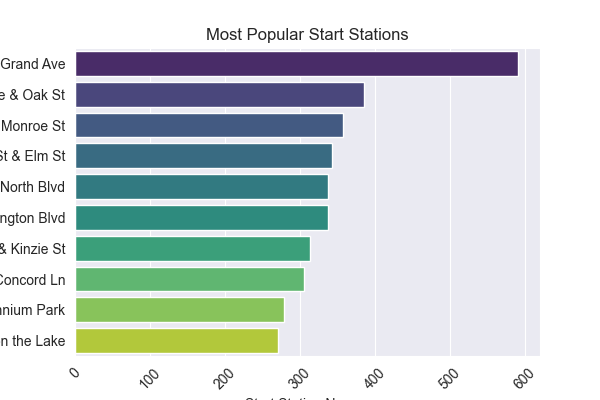
\includegraphics[width=0.8\textwidth]{images/count_most_popular_start_stations}
        \caption{Annual Data Trend}
        \label{fig:graph1}
    \end{figure}


    \section*{Dataset description}
    \label{sec:dataset}

    \subsection{Dataset Features}\label{subsec:dataset-features}
    \begin{itemize}
        \item \textbf{star\_ride\_id}: A unique identifier for each trip, ensuring individual trips can be tracked and analyzed discretely.
        \item \textbf{star\_rideable\_type}: The type of bike used for the trip, which can influence usage patterns and availability needs.
        \item \textbf{star\_started\_at}: The timestamp indicating when a trip started, crucial for understanding demand over time.
        \item \textbf{star\_ended\_at}: The timestamp indicating when a trip ended, allowing for the calculation of trip duration and temporal patterns of bike usage.
        \item \textbf{star\_start\_station\_name}: The name of the station where the trip originated, providing a geographic point for demand analysis.
        \item \textbf{star\_start\_station\_id}: A unique identifier for the origin station, which can be used in conjunction with geographic data for mapping and spatial analysis.
        \item \textbf{star\_end\_station\_name}: The name of the station where the trip concluded, indicating the destination demand in the network.
        \item \textbf{star\_end\_station\_id}: A unique identifier for the destination station, useful for spatial analysis and redistribution strategies.
        \item \textbf{star\_start\_lat \& start\_lng}: The latitude and longitude of the start station, giving precise location data for origin points.
        \item \textbf{star\_end\_lat \& end\_lng}: The latitude and longitude of the end station, giving precise location data for destination points.
        \item \textbf{star\_member\_casual}: A categorization of the user as a member or a casual rider, which can influence riding patterns and frequency of use.
    \end{itemize}

    \subsection{Added Features}\label{subsec:added-features}
    \begin{itemize}
        \item \textbf{week\_day\_index}: Categorised into Morning, Afternoon, Evening, and Night, to analyse demand fluctuations.
        \item \textbf{day\_period\_index}: Classified into working and non-working days, to observe weekly patterns in bike usage.
    \end{itemize}

    While the focus is not on text processing, storing text-based features like station names and user types enriches data visualisation, making it more accessible and interpretable. This approach, although not critical for data model training, enhances the user experience during data exploration.
    \textbf{Importance of Accessibility:} \newline
    A dataset's value is significantly enhanced by its accessibility.
    By detailing and explaining the dataset's features, this report aims to ensure that the data is as useful and informative as possible for the intended analysis.

    \begin{thebibliography}{99} % '99' here is a placeholder that adjusts based on the widest label

        \bibitem{DivvyData}
        DivvyData, ``Bike ride-sharing data,'' 2023. [Online]. Available: \url{https://divvybikes.com/system-data}

        \bibitem{DataSource}
        DivvyData Dataset, ``Index file for historic data,'' 2023. [Online]. Available: \url{https://divvy-tripdata.s3.amazonaws.com/index.html}

        \bibitem{2016}
        J. Zhang, X. Pan, M. Li, and P. S. Yu, ``Bicycle-Sharing System Analysis and Trip Prediction,'' in \textit{2016 17th IEEE International Conference on Mobile Data Management (MDM)}, vol. 1, pp. 174-179, 2016. DOI: \href{https://doi.org/10.1109/MDM.2016.35}{10.1109/MDM.2016.35}

        \bibitem{2015}
        Y. Li, Y. Zheng, H. Zhang, and L. Chen, ``Traffic prediction in a bike-sharing system,'' \textit{Proceedings of the 23rd SIGSPATIAL International Conference on Advances in Geographic Information Systems}, SIGSPATIAL '15, New York, NY, USA: Association for Computing Machinery, 2015, Art. no. 33. DOI: \href{https://doi.org/10.1145/2820783.2820837}{10.1145/2820783.2820837}

        \bibitem{s18020512}
        F. Chiariotti, C. Pielli, A. Zanella, and M. Zorzi, ``A Dynamic Approach to Rebalancing Bike-Sharing Systems,'' \textit{Sensors}, vol. 18, no. 2, Art. no. 512, 2018. DOI: \href{https://www.mdpi.com/1424-8220/18/2/512}{10.3390/s18020512}

    \end{thebibliography}
\end{document}
